\subsection{Interface graph}

Библиотека Roren включает в себя несколько абстракций, которые упрощают процесс обработки данных в условиях больших распределенных систем. Эти абстракции применимы как к batch, так и к streaming источникам данных. При создании pipeline-а есть возможность структурировать задачи обработки данных, используя абстракции преобразований данных и результатов их применений - transform-ов и collection-ов соответственно.

Pipeline описывает всю задачу обработки данных от начала до конца. Он включает в себя чтение входных данных, их преобразование и запись выходных таблиц. При его создании есть возможность указать параметры выполнения, специфичные для конкретного паттерна выполнения: настройки streaming или MapReduce инфраструктуры.

Collection представляет собой распределенный набор данных, с которым работает pipeline. Набор данных может быть ограниченным, то есть происходить из фиксированного источника, как файл, или неограниченным, то есть поступать из постоянно обновляющегося streaming источника. Типичный pipeline создает начальный collection, читая данные из внешнего источника данных. Далее, коллекции служат входными и выходными данными для каждого преобразования в pipeline.

Transform представляет операцию обработки данных. Каждый transform принимает один или несколько объектов collection в качестве входных данных, выполняет функцию обработки, которую пользователь предоставляет, над элементами этой коллекции данных, а затем производит ноль (в случае стока графа - записи во внешнее хранилище) или более выходных объектов collection.

Roren включает множество I/O преобразований - библиотечных transforms, которые читают или записывают данные в различные внешние системы хранения данных. Чтения и записи таблиц в случае MapReduce или топиков брокеров сообщений осуществляются через общие интерфейсы IRawRead и IRawWrite.

Трансформации могут изменять, фильтровать, группировать, анализировать или иным образом обрабатывать элементы collection-а. Преобразование создает новую выходную коллекцию данных, не модифицируя входную коллекцию. Типичный pipeline применяет последующие трансформации к каждой новой выходной collection по очереди, пока обработка не будет завершена. Однако стоит отметить, что пайплайн не обязательно должен быть одной прямой линией трансформаций, применяемых одна за другой. Можно рассматривать коллекции как переменные, а преобразования как функции, применяемые к этим переменным, что позволяет создать сложный граф обработки.

После того, как в коде описаны все transform-ы, pipeline запускается с использованием назначенного executor-а (рис~\ref{fig:pipeline}).

\begin{figure}[h]
    \centering
    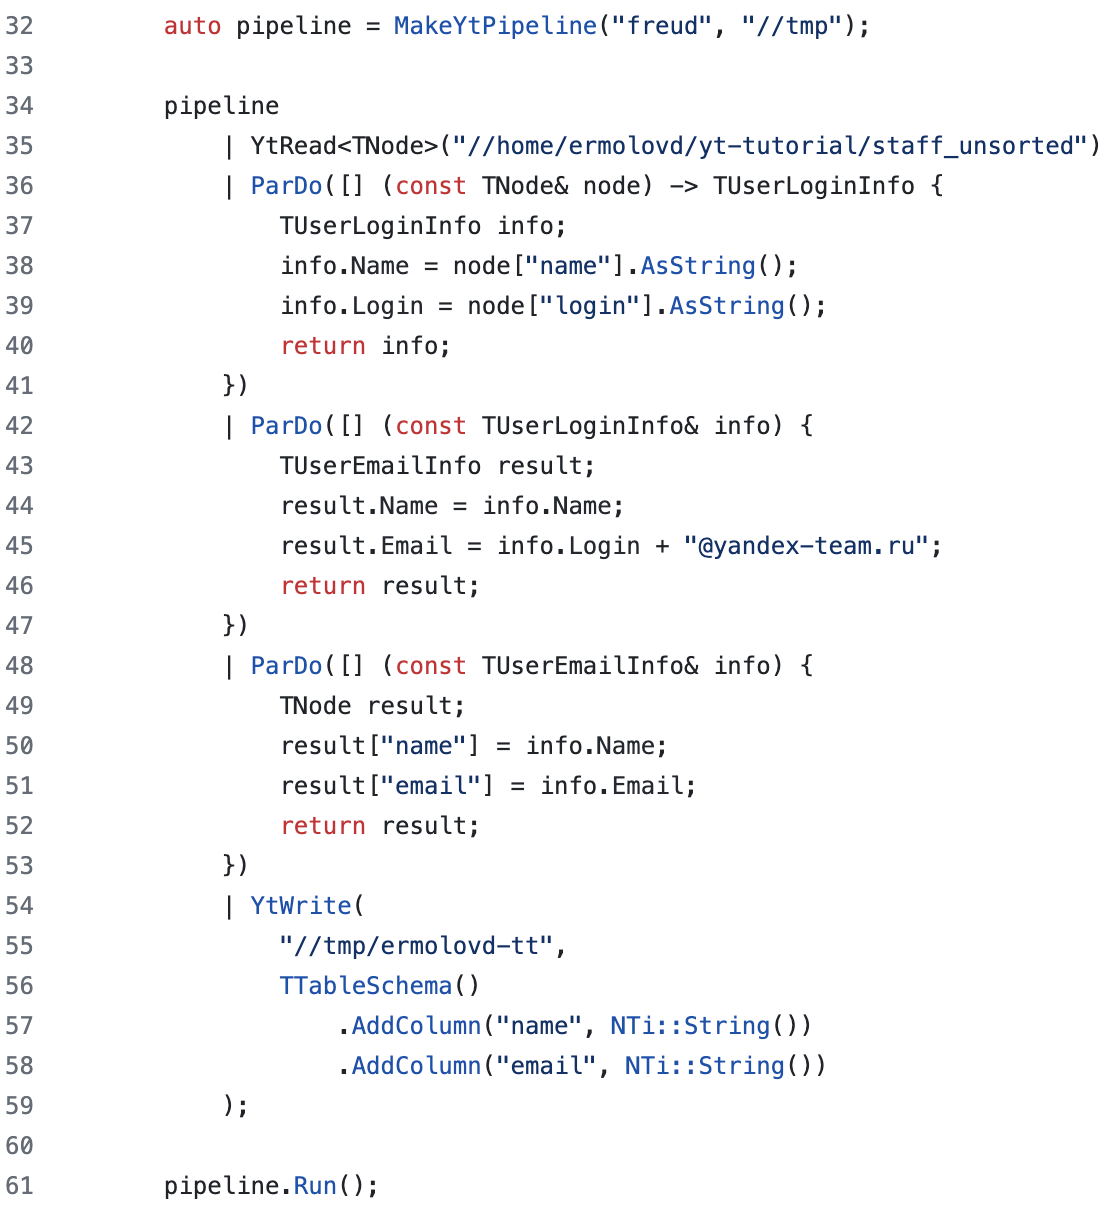
\includegraphics[width=\textwidth]{img/pipeline.png}
    \caption{Типичный pipeline с YT executor-ом}
    \label{fig:pipeline}
\end{figure}
